%%\VignetteEngine{knitr::knitr}
%%\VignetteIndexEntry{Using proftools}
\documentclass[nojss]{jss}\usepackage[]{graphicx}\usepackage[]{color}
%% maxwidth is the original width if it is less than linewidth
%% otherwise use linewidth (to make sure the graphics do not exceed the margin)
\makeatletter
\def\maxwidth{ %
  \ifdim\Gin@nat@width>\linewidth
    \linewidth
  \else
    \Gin@nat@width
  \fi
}
\makeatother

\definecolor{fgcolor}{rgb}{0.345, 0.345, 0.345}
\newcommand{\hlnum}[1]{\textcolor[rgb]{0.686,0.059,0.569}{#1}}%
\newcommand{\hlstr}[1]{\textcolor[rgb]{0.192,0.494,0.8}{#1}}%
\newcommand{\hlcom}[1]{\textcolor[rgb]{0.678,0.584,0.686}{\textit{#1}}}%
\newcommand{\hlopt}[1]{\textcolor[rgb]{0,0,0}{#1}}%
\newcommand{\hlstd}[1]{\textcolor[rgb]{0.345,0.345,0.345}{#1}}%
\newcommand{\hlkwa}[1]{\textcolor[rgb]{0.161,0.373,0.58}{\textbf{#1}}}%
\newcommand{\hlkwb}[1]{\textcolor[rgb]{0.69,0.353,0.396}{#1}}%
\newcommand{\hlkwc}[1]{\textcolor[rgb]{0.333,0.667,0.333}{#1}}%
\newcommand{\hlkwd}[1]{\textcolor[rgb]{0.737,0.353,0.396}{\textbf{#1}}}%

\usepackage{framed}
\makeatletter
\newenvironment{kframe}{%
 \def\at@end@of@kframe{}%
 \ifinner\ifhmode%
  \def\at@end@of@kframe{\end{minipage}}%
  \begin{minipage}{\columnwidth}%
 \fi\fi%
 \def\FrameCommand##1{\hskip\@totalleftmargin \hskip-\fboxsep
 \colorbox{shadecolor}{##1}\hskip-\fboxsep
     % There is no \\@totalrightmargin, so:
     \hskip-\linewidth \hskip-\@totalleftmargin \hskip\columnwidth}%
 \MakeFramed {\advance\hsize-\width
   \@totalleftmargin\z@ \linewidth\hsize
   \@setminipage}}%
 {\par\unskip\endMakeFramed%
 \at@end@of@kframe}
\makeatother

\definecolor{shadecolor}{rgb}{.97, .97, .97}
\definecolor{messagecolor}{rgb}{0, 0, 0}
\definecolor{warningcolor}{rgb}{1, 0, 1}
\definecolor{errorcolor}{rgb}{1, 0, 0}
\newenvironment{knitrout}{}{} % an empty environment to be redefined in TeX

\usepackage{alltt}

%%%%%%%%%%%%%%%%%%%%%%%%%%%%%%
%% declarations for jss.cls %%%%%%%%%%%%%%%%%%%%%%%%%%%%%%%%%%%%%%%%%%
%%%%%%%%%%%%%%%%%%%%%%%%%%%%%%

%% almost as usual
\author{Luke Tierney\\University of Iowa \And 
        Riad Jarjour\\University of Iowa}
\title{Examining \proglang{R} Profiling Data: The \pkg{proftools} Package}

%% for pretty printing and a nice hypersummary also set:
\Plainauthor{Luke Tierney, Riad Jarjour} %% comma-separated
\Plaintitle{Examining R Profiling Data:
  The proftools Package} %% without formatting
%$ \Shorttitle{\pkg{foo}: A Capitalized Title} %% a short title (if necessary)

%% an abstract and keywords
\Abstract{
  This note introduces the \pkg{proftools} package for
  examining data collected by \proglang{R}'s sampling profiler.
  \pkg{proftools} includes facilities for summarizing results at the
  function, call, and source line level; for filtering to narrow the
  focus to functions of primary interest; and for visualizing
  profiling data. Use of the package is illustrated with a small
  running example.
}
\Keywords{\pkg{proftools}, profiling, \proglang{R}, \code{Rprof}}
\Plainkeywords{proftools, profiling, R, Rprof} %% without formatting
%% at least one keyword must be supplied

%% publication information
%% NOTE: Typically, this can be left commented and will be filled out by the technical editor
%% \Volume{50}
%% \Issue{9}
%% \Month{June}
%% \Year{2012}
%% \Submitdate{2012-06-04}
%% \Acceptdate{2012-06-04}

%% The address of (at least) one author should be given
%% in the following format:
\Address{
  Luke Tierney\\
  Department of Statistics and Actuarial Science\\
  Faculty of Statistics\\
  University of Iowa\\
  Iowa City, USA\\
  E-mail: \email{luke-tierney@uiowa.edu}\\
  URL: \url{http://homepage.stat.uiowa.edu/~luke/}
  
  Riad Jarjour\\
  Department of Statistics and Actuarial Science\\
  Faculty of Statistics\\
  University of Iowa\\
  Iowa City, USA\\
  E-mail: \email{riad-jarjour@uiowa.edu}
}
%% It is also possible to add a telephone and fax number
%% before the e-mail in the following format:
%% Telephone: +43/512/507-7103
%% Fax: +43/512/507-2851

%% for those who use Sweave please include the following line (with % symbols):
%% need no \usepackage{Sweave.sty}

%% end of declarations %%%%%%%%%%%%%%%%%%%%%%%%%%%%%%%%%%%%%%%%%%%%%%%
\IfFileExists{upquote.sty}{\usepackage{upquote}}{}
\begin{document}

%% include your article here, just as usual
%% Note that you should use the \pkg{}, \proglang{} and <<>>=} commands.

\section{Introduction}

Profiling is a program analysis method for determining where a program
run spends most of its execution time, and can be very helpful in
guiding programmer effort for improving program performance.
\proglang{R} includes a sampling based profiling mechanism that
records information about calls on the stack at specified time
intervals.  If available, information about the specific source code
lines active at the sampling point is recorded as well. Information
about time spent in the garbage collector can also be collected. The
collected profiling data is written to a file, by default the file
\code{Rprof.out} in the current working directory.  The function
\code{summaryRprof}, available in the \pkg{base} package in
\proglang{R}, provides a simple interface for examining this data. The
\pkg{proftools} package provides a much more extensive set of tools
for summarizing, visualizing, and filtering this data.

\section{Collecting Profile Data}
The \pkg{proftools} package includes an example script \code{bootlm.R}
in the \code{samples} directory that runs several examples from the
\pkg{boot} package \citep{CantyRipley:Boot} and then fits a simple
linear model. The file path can be obtained as
\begin{knitrout}\small
\definecolor{shadecolor}{rgb}{0.969, 0.969, 0.969}\color{fgcolor}\begin{kframe}
\begin{alltt}
\hlstd{srcfile} \hlkwb{<-} \hlkwd{system.file}\hlstd{(}\hlstr{"samples"}\hlstd{,} \hlstr{"bootlmEx.R"}\hlstd{,} \hlkwc{package} \hlstd{=} \hlstr{"proftools"}\hlstd{)}
\end{alltt}
\end{kframe}
\end{knitrout}

The traditional way to collect profiling data in R is to call
\code{Rprof} to start profiling, run the code to be profiled, and then
call \code{Rprof} again to end profiling. For example, to profile the
code in \code{bootlm.R}, and collect both source line and GC
information, you could use
\begin{knitrout}\small
\definecolor{shadecolor}{rgb}{0.969, 0.969, 0.969}\color{fgcolor}\begin{kframe}
\begin{alltt}
\hlstd{profout} \hlkwb{<-} \hlkwd{tempfile}\hlstd{()}
\hlkwd{Rprof}\hlstd{(}\hlkwc{file} \hlstd{= profout,} \hlkwc{gc.profiling} \hlstd{=} \hlnum{TRUE}\hlstd{,} \hlkwc{line.profiling} \hlstd{=} \hlnum{TRUE}\hlstd{)}
\hlkwd{source}\hlstd{(srcfile)}
\hlkwd{Rprof}\hlstd{(}\hlkwa{NULL}\hlstd{)}
\hlstd{pd} \hlkwb{<-} \hlkwd{readProfileData}\hlstd{(profout)}
\hlkwd{unlink}\hlstd{(profout)}
\end{alltt}
\end{kframe}
\end{knitrout}
The \pkg{proftools} package provides the simpler alternative
\begin{knitrout}\small
\definecolor{shadecolor}{rgb}{0.969, 0.969, 0.969}\color{fgcolor}\begin{kframe}
\begin{alltt}
\hlstd{pd} \hlkwb{<-} \hlkwd{profileExpr}\hlstd{(}\hlkwd{source}\hlstd{(srcfile))}
\end{alltt}
\end{kframe}
\end{knitrout}
By default \code{profileExpr} enables GC and source information to be
collected. It also trims off stack information leading up to the
\code{profileExpr} call.

\section{Summary Functions}
The most basic summary function is \code{funSummary} for summarizing
profile results at the function level. It produces information similar
to the result returned by R's \code{summaryRprof} but in a more usable
form:
\begin{knitrout}\small
\definecolor{shadecolor}{rgb}{0.969, 0.969, 0.969}\color{fgcolor}\begin{kframe}
\begin{alltt}
\hlkwd{head}\hlstd{(}\hlkwd{funSummary}\hlstd{(pd),} \hlnum{10}\hlstd{)}
\end{alltt}
\begin{verbatim}
##                      total.pct gc.pct self.pct gcself.pct
## withVisible             100.00   9.00     0.00       0.00
## source                  100.00   9.00     0.00       0.00
## eval                    100.00   9.00     0.71       0.00
## statistic                78.20   4.03     0.00       0.00
## lapply                   78.20   4.03     0.71       0.00
## FUN                      78.20   4.03     1.66       0.24
## glm (bootlmEx.R:33)      50.47   1.90     0.00       0.00
## boot (bootlmEx.R:39)     37.68   2.84     0.00       0.00
## boot (bootlmEx.R:44)     36.73   1.18     0.00       0.00
## sapply                   31.99   2.37     0.71       0.00
\end{verbatim}
\end{kframe}
\end{knitrout}
The result returned by \code{funSummary}, and most summary functions,
is a data frame, so \code{head} can be used to focus on the top
entries. 

By default, when source information is available results are
summarized at the call level, so multiple calls to \code{boot} from
different source lines are shown separately. This can be suppressed by
supplying the \code{srclines = FALSE} argument:
\begin{knitrout}\small
\definecolor{shadecolor}{rgb}{0.969, 0.969, 0.969}\color{fgcolor}\begin{kframe}
\begin{alltt}
\hlkwd{head}\hlstd{(}\hlkwd{funSummary}\hlstd{(pd,} \hlkwc{srclines} \hlstd{=} \hlnum{FALSE}\hlstd{),} \hlnum{10}\hlstd{)}
\end{alltt}
\begin{verbatim}
##                     total.pct gc.pct self.pct gcself.pct
## withVisible            100.00   9.00     0.00       0.00
## source                 100.00   9.00     0.00       0.00
## eval                   100.00   9.00     0.71       0.00
## statistic               78.20   4.03     0.00       0.00
## lapply                  78.20   4.03     0.71       0.00
## FUN                     78.20   4.03     1.66       0.24
## boot                    78.20   4.03     0.00       0.00
## glm                     50.47   1.90     0.00       0.00
## sapply                  31.99   2.37     0.71       0.00
## model.frame.default     30.33   2.61     1.66       0.00
\end{verbatim}
\end{kframe}
\end{knitrout}

Data can also be summarized by call:
\begin{knitrout}\small
\definecolor{shadecolor}{rgb}{0.969, 0.969, 0.969}\color{fgcolor}\begin{kframe}
\begin{alltt}
\hlkwd{head}\hlstd{(}\hlkwd{callSummary}\hlstd{(pd),} \hlnum{10}\hlstd{)}
\end{alltt}
\begin{verbatim}
##                                  total.pct gc.pct self.pct gcself.pct
## withVisible -> eval                 100.00   9.00     0.00          0
## source -> withVisible               100.00   9.00     0.00          0
## eval -> eval                        100.00   9.00     0.24          0
## lapply -> FUN                        78.20   4.03     0.71          0
## FUN -> statistic                     77.96   3.79     0.00          0
## statistic -> glm (bootlmEx.R:33)     50.47   1.90     0.00          0
## eval -> boot (bootlmEx.R:39)         37.68   2.84     0.00          0
## boot (bootlmEx.R:39) -> lapply       37.44   2.61     0.00          0
## eval -> boot (bootlmEx.R:44)         36.73   1.18     0.00          0
## boot (bootlmEx.R:44) -> lapply       36.73   1.18     0.00          0
\end{verbatim}
\end{kframe}
\end{knitrout}

When source information is available in the profile data the
\code{srcSummary} function can be used to summarize at the source line
level; only lines appearing in the sample are included:
\begin{knitrout}\small
\definecolor{shadecolor}{rgb}{0.969, 0.969, 0.969}\color{fgcolor}\begin{kframe}
\begin{alltt}
\hlkwd{srcSummary}\hlstd{(pd)}
\end{alltt}
\begin{verbatim}
##               total.pct gctotal.pct                              source
## bootlmEx.R:8       2.61        0.00     gp1 <- 1:table(as.numeric(d ...
## bootlmEx.R:9       0.24        0.00     m1 <- sum(d[gp1,1] * f[gp1] ...
## bootlmEx.R:11      0.47        0.00     ss1 <- sum(d[gp1,1]^2 * f[g ...
## bootlmEx.R:12      0.47        0.00     ss2 <- sum(d[-gp1,1]^2 * f[ ...
## bootlmEx.R:16      3.79        0.00 boot(grav1, diff.means, R = 999 ...
## bootlmEx.R:33     50.47        1.90     lm.b <- glm(fit+resid[inds] ...
## bootlmEx.R:35     23.70        2.13     pred.b <- predict(lm.b, x.pred)
## bootlmEx.R:36      0.24        0.00     c(coef(lm.b), pred.b - (fit ...
## bootlmEx.R:39     37.68        2.84 nuke.boot <- boot(nuke.data, nu ...
## bootlmEx.R:44     36.73        1.18 nuke.boot <- boot(nuke.data, nu ...
## bootlmEx.R:50      6.87        0.71 X <- matrix(rnorm(n * p), n, p)    
## bootlmEx.R:51      0.47        0.00 y <- rnorm(n) + X[,1]              
## bootlmEx.R:52     14.45        4.27 fit <- lm(y ~ X)
\end{verbatim}
\end{kframe}
\end{knitrout}
The function \code{annotateSource} can show the full files with
profiling annotations.

A useful way to examine profile data is to look for hot execution
paths.  This approach sorts functions called at top level, i.e. at the
bottom of the call stack, by the total amount of time spent in their
top level calls; within each top level call to a function \code{f} the
functions called by \code{f} are sorted by the amount of time spent in
them within the top level call to \code{f}; and the process continues
for higher level calls. The function \code{hotPaths} produces a hot
path summary; the \code{total.pct} argument causes leaf functions in
stack traces to be pruned back until the execution time percentage for
each stack trace is at least \code{total.pct}:
\begin{knitrout}\small
\definecolor{shadecolor}{rgb}{0.969, 0.969, 0.969}\color{fgcolor}\begin{kframe}
\begin{alltt}
\hlkwd{hotPaths}\hlstd{(pd,} \hlkwc{total.pct} \hlstd{=} \hlnum{10.0}\hlstd{)}
\end{alltt}
\begin{verbatim}
##  path                                    total.pct self.pct
##  source                                  100.00     0.00   
##  . withVisible                           100.00     0.00   
##  . . eval                                100.00     0.00   
##  . . . eval                              100.00     0.00   
##  . . . . boot (bootlmEx.R:39)             37.68     0.00   
##  . . . . . lapply                         37.44     0.00   
##  . . . . . . FUN                          37.44     0.00   
##  . . . . . . . statistic                  37.44     0.00   
##  . . . . . . . . glm (bootlmEx.R:33)      24.88     0.00   
##  . . . . . . . . . eval                   11.85    11.85   
##  . . . . . . . . predict (bootlmEx.R:35)  12.32     0.00   
##  . . . . . . . . . predict.glm            12.32    12.32   
##  . . . . boot (bootlmEx.R:44)             36.73     0.00   
##  . . . . . lapply                         36.73     0.00   
##  . . . . . . FUN                          36.73     0.00   
##  . . . . . . . statistic                  36.73     0.00   
##  . . . . . . . . glm (bootlmEx.R:33)      25.59     0.00   
##  . . . . . . . . . eval                   13.03    13.03   
##  . . . . . . . . predict (bootlmEx.R:35)  11.14     0.00   
##  . . . . . . . . . predict.glm            11.14    11.14   
##  . . . . lm (bootlmEx.R:52)               14.45     0.00
\end{verbatim}
\end{kframe}
\end{knitrout}
Examining the result of \code{hotPaths} starting with high values of
\code{total.pct} and then moving to lower values is a useful way to
explore where the computational effort is concentrated.  An alternative
for limiting the depth to which stack traces are followed is provided
by the \code{maxdepth} argument.
%% Other summary: \code{pathSummary}

\section{Filtering Profile Data}
The hot path summary shows information associated with the source
command itself that is not directly relevant to our analysis. The
\code{filterProfileData} function can be uses to select or omit
certain functions, drop functions with small self or total times,
narrow to a particular time interval, among others.  For example, by
selecting only stack traces that include calls to \code{withVisible}
and then trimming off the leading four calls we can focus just on the
work done in the sourced file:
\begin{knitrout}\small
\definecolor{shadecolor}{rgb}{0.969, 0.969, 0.969}\color{fgcolor}\begin{kframe}
\begin{alltt}
\hlstd{filteredPD} \hlkwb{<-} \hlkwd{filterProfileData}\hlstd{(pd,} \hlkwc{select} \hlstd{=} \hlstr{"withVisible"}\hlstd{,} \hlkwc{skip} \hlstd{=} \hlnum{4}\hlstd{)}
\end{alltt}
\end{kframe}
\end{knitrout}
The hot path summary for this reduced profile is
\begin{knitrout}\small
\definecolor{shadecolor}{rgb}{0.969, 0.969, 0.969}\color{fgcolor}\begin{kframe}
\begin{alltt}
\hlkwd{hotPaths}\hlstd{(filteredPD,} \hlkwc{total.pct} \hlstd{=} \hlnum{10.0}\hlstd{)}
\end{alltt}
\begin{verbatim}
##  path                            total.pct self.pct
##  boot (bootlmEx.R:39)            37.68     0.00    
##  . lapply                        37.44     0.00    
##  . . FUN                         37.44     0.00    
##  . . . statistic                 37.44     0.00    
##  . . . . glm (bootlmEx.R:33)     24.88     0.00    
##  . . . . . eval                  11.85     0.00    
##  . . . . . . eval                11.85     0.00    
##  . . . . predict (bootlmEx.R:35) 12.32     0.00    
##  . . . . . predict.glm           12.32     0.00    
##  . . . . . . predict.lm          11.85     0.00    
##  boot (bootlmEx.R:44)            36.73     0.00    
##  . lapply                        36.73     0.00    
##  . . FUN                         36.73     0.00    
##  . . . statistic                 36.73     0.00    
##  . . . . glm (bootlmEx.R:33)     25.59     0.00    
##  . . . . . eval                  13.03     0.24    
##  . . . . . . eval                12.80     0.00    
##  . . . . predict (bootlmEx.R:35) 11.14     0.00    
##  . . . . . predict.glm           11.14     0.24    
##  . . . . . . predict.lm          10.43     0.71    
##  lm (bootlmEx.R:52)              14.45     0.00
\end{verbatim}
\end{kframe}
\end{knitrout}

We can use the \code{focus} filter to further narrow our examination
to stack frames containing calls to \code{glm} and also remove all
calls preceding the first \code{glm} call from the selected stack
frames. For this reduced data it also makes sense to follow the paths
further by lowering \code{total.pct} to 5\%:
\begin{knitrout}\small
\definecolor{shadecolor}{rgb}{0.969, 0.969, 0.969}\color{fgcolor}\begin{kframe}
\begin{alltt}
\hlstd{glmPD} \hlkwb{<-} \hlkwd{filterProfileData}\hlstd{(filteredPD,} \hlkwc{focus} \hlstd{=} \hlstr{"glm"}\hlstd{)}
\hlkwd{hotPaths}\hlstd{(glmPD,} \hlkwc{total.pct} \hlstd{=} \hlnum{5.0}\hlstd{)}
\end{alltt}
\begin{verbatim}
##  path                             total.pct self.pct
##  glm (bootlmEx.R:33)              50.47     0.00    
##  . eval                           24.88     0.24    
##  . . eval                         24.64     0.00    
##  . . . <Anonymous>                18.01     0.00    
##  . . . . model.frame.default      18.01     0.71    
##  . . . . . sapply                  7.35     0.24    
##  . . . . . . lapply                6.16     0.24    
##  . . . . . . . FUN                 5.92     0.00    
##  . . . . . . . . paste             5.92     0.47    
##  . . . . . . . . . deparse         5.45     5.45    
##  . . . . . .External2              5.92     0.00    
##  . . . . . . na.omit               5.92     0.00    
##  . . . . . . . na.omit.data.frame  5.92     0.95    
##  . . . glm.fit                     6.40     3.08    
##  . model.matrix                   12.32     0.24    
##  . . model.matrix.default         12.09     1.18    
##  . . . match                       8.29     0.00    
##  . . . . sapply                    8.29     0.00    
##  . . . . . lapply                  7.82     0.00    
##  . . . . . . FUN                   7.58     0.00    
##  . . . . . . . paste               7.58     1.18    
##  . . . . . . . . deparse           6.40     1.66    
##  . .getXlevels                     8.29     0.24    
##  . . sapply                        5.21     0.00
\end{verbatim}
\end{kframe}
\end{knitrout}


\section{Visualizing Profile Data}
\href{https://en.wikipedia.org/wiki/Call_graph}{Call graphs} annotated
with profile information are a very popular way to view profiling
results.  \code{plotProfileCallGraph} uses the \pkg{graph}
\citep{Gentleman:graph} and \pkg{Rgraphviz} \citep{Gentry:Rgraphviz}
packages from Bioconductor to render an annotated call graph. The
default style for the graph is based on the style used in
\href{https://github.com/gperftools}{Google's profiling library} but
can be customized in a number of ways.  A call graph for the full
profile data is produced by
\begin{knitrout}\small
\definecolor{shadecolor}{rgb}{0.969, 0.969, 0.969}\color{fgcolor}\begin{kframe}
\begin{alltt}
\hlkwd{plotProfileCallGraph}\hlstd{(pd)}
\end{alltt}
\end{kframe}\begin{figure}

{\centering \includegraphics[width=\maxwidth]{figure/fullCallGraph-1} 

}

\caption[Full call graph of profile data]{Full call graph of profile data.}\label{fig:fullCallGraph}
\end{figure}


\end{knitrout}
and is shown in Figure \ref{fig:fullCallGraph}.

By default the call graph size is limited to at most 30 nodes; nodes
with lower total hit counts are dropped. The \code{maxnodes} argument
can be used to adjust this limit. Also by default color is used to
encode the total hit score for the function nodes. This can be
suppressed with the \code{score = "none"} argument.

We can obtain a more readable graph by filtering. For example, to
examine the \code{glm.fit} call and its callees we can use
\begin{knitrout}\small
\definecolor{shadecolor}{rgb}{0.969, 0.969, 0.969}\color{fgcolor}\begin{kframe}
\begin{alltt}
\hlkwd{plotProfileCallGraph}\hlstd{(}\hlkwd{filterProfileData}\hlstd{(pd,} \hlkwc{focus} \hlstd{=} \hlstr{"glm.fit"}\hlstd{))}
\end{alltt}
\end{kframe}\begin{figure}

{\centering \includegraphics[width=\maxwidth]{figure/filteredCallGraph-1} 

}

\caption{Call graph for \code{glm.fit} call.}\label{fig:filteredCallGraph}
\end{figure}


\end{knitrout}
The result is shown in Figure \ref{fig:filteredCallGraph}.

A printed version of the call graph, similar to the call graph
produced by \code{gprof} \citep{Graham:1982:GCG:800230.806987}, can be
obtained with \code{printProfileCallGraph}.  For the subgraph of the
\code{glm.fit} calls, for example,
\begin{knitrout}\small
\definecolor{shadecolor}{rgb}{0.969, 0.969, 0.969}\color{fgcolor}\begin{kframe}
\begin{alltt}
\hlkwd{printProfileCallGraph}\hlstd{(}\hlkwd{filterProfileData}\hlstd{(pd,} \hlkwc{focus} \hlstd{=} \hlstr{"glm.fit"}\hlstd{))}
\end{alltt}
\end{kframe}
\end{knitrout}
produces the printed representation shown in Figure \ref{fig:printGraph}.
\begin{figure}
  \tiny
\begin{knitrout}\small
\definecolor{shadecolor}{rgb}{0.969, 0.969, 0.969}\color{fgcolor}\begin{kframe}
\begin{verbatim}
Call graph

index    % time     % self   % children     name

[1]        6.40       3.08       3.32     glm.fit [1]    
                      0.47       0.00         $ [3] 
                      0.24       0.00         [Anonymous] [7] 
                      0.24       0.00         as.matrix [8] 
                      0.95       0.00         .Call [2] 
                      0.00       0.47         do.call [4] 
                      0.24       0.00         is.finite [10] 
                      0.24       0.00         rep.int [6] 
                      0.00       0.24         structure [12] 
                      0.00       0.24         variance [13] 
-----------------------------------------------
                      0.95       0.00         glm.fit [1] 
[2]        0.95       0.95       0.00     .Call [2]    
-----------------------------------------------
                      0.47       0.00         glm.fit [1] 
[3]        0.47       0.47       0.00     $ [3]    
-----------------------------------------------
                      0.00       0.47         glm.fit [1] 
[4]        0.47       0.00       0.47     do.call [4]    
                      0.47       0.00         glm.control [5] 
-----------------------------------------------
                      0.47       0.00         do.call [4] 
[5]        0.47       0.47       0.00     glm.control [5]    
-----------------------------------------------
                      0.24       0.00         variance [13] 
                      0.24       0.00         glm.fit [1] 
[6]        0.47       0.47       0.00     rep.int [6]    
-----------------------------------------------
                      0.24       0.00         glm.fit [1] 
[7]        0.24       0.24       0.00     [Anonymous] [7]    
-----------------------------------------------
                      0.24       0.00         glm.fit [1] 
[8]        0.24       0.24       0.00     as.matrix [8]    
-----------------------------------------------
                      0.00       0.24         structure [12] 
[9]        0.24       0.00       0.24     %in% [9]    
                      0.24       0.00         match [11] 
-----------------------------------------------
                      0.24       0.00         glm.fit [1] 
[10]       0.24       0.24       0.00     is.finite [10]   
-----------------------------------------------
                      0.24       0.00         %in% [9] 
[11]       0.24       0.24       0.00     match [11]   
-----------------------------------------------
                      0.00       0.24         glm.fit [1] 
[12]       0.24       0.00       0.24     structure [12]   
                      0.00       0.24         %in% [9] 
-----------------------------------------------
                      0.00       0.24         glm.fit [1] 
[13]       0.24       0.00       0.24     variance [13]   
                      0.24       0.00         rep.int [6] 
-----------------------------------------------
\end{verbatim}
\end{kframe}
\end{knitrout}
\caption{Printed call graph.}
\label{fig:printGraph}
\end{figure}

Another visualization sometimes used is a
\href{http://www.brendangregg.com/flamegraphs.html}{flame graph}. A flame graph for the original data is produced by
\begin{knitrout}\small
\definecolor{shadecolor}{rgb}{0.969, 0.969, 0.969}\color{fgcolor}\begin{kframe}
\begin{alltt}
\hlkwd{flameGraph}\hlstd{(pd)}
\end{alltt}
\end{kframe}\begin{figure}

{\centering \includegraphics[width=4in]{figure/flameGraph-1} 

}

\caption[Flame graph visualizing hot paths for the full profile data]{Flame graph visualizing hot paths for the full profile data.}\label{fig:flameGraph}
\end{figure}


\end{knitrout}
The result is shown in Figure \ref{fig:flameGraph}.  A flame graph of
the filtered data is produced by
\begin{knitrout}\small
\definecolor{shadecolor}{rgb}{0.969, 0.969, 0.969}\color{fgcolor}\begin{kframe}
\begin{alltt}
\hlkwd{flameGraph}\hlstd{(filteredPD)}
\end{alltt}
\end{kframe}\begin{figure}

{\centering \includegraphics[width=4in]{figure/filteredFlameGraph-1} 

}

\caption[Flame graph of the filtered profile data]{Flame graph of the filtered profile data.}\label{fig:filteredFlameGraph}
\end{figure}


\end{knitrout}
and shown in Figure \ref{fig:filteredFlameGraph}
%% Furthermore, an svg file of the graph can be outputted by using the
%% svg argument:
%% <<eval=FALSE>>=
%% flameGraph(pd, svg = "graph.svg", order = "hot")
%% @ 

The vertical positions of rectangles in these flame graphs represent
call depth on the stack. The widths of the rectangles represent the
amount of time spent in a call at a particular call or set of calls at
a particular depth. The \code{order} argument determines the ordering
of call rectangles at a particular level within a call at the lower
level. The default order is \code{"hot"}; it uses the hot path
ordering with the call with the largest amount of time first.  This
produces a visual representation of the hot path summary.  The
\code{"alpha"} ordering orders the calls alphabetically.

Specifying \code{order = "time"} shows the calls in the order in which
they occurred:
\begin{knitrout}\small
\definecolor{shadecolor}{rgb}{0.969, 0.969, 0.969}\color{fgcolor}\begin{kframe}
\begin{alltt}
\hlkwd{flameGraph}\hlstd{(pd,} \hlkwc{order} \hlstd{=} \hlstr{"time"}\hlstd{)}
\end{alltt}
\end{kframe}\begin{figure}

{\centering \includegraphics[width=4in]{figure/timeGraph-1} 

}

\caption[Time graph of the full profile data]{Time graph of the full profile data.}\label{fig:timeGraph}
\end{figure}


\end{knitrout}
Figure \ref{fig:timeGraph} shows the \code{boot} calls preceding the
data generation for the \code{lm} call and the \code{lm} call itself.

Default colors for flame graphs are based on the \code{rainbow}
palette. Alternative colors can be specified by providing a
\code{colormap} function. If space permits, the call labels are
printed within the rectangles representing the calls. A method for the
\code{identify} function is available that can be used to identify the
individual calls when they are not visible. An option to this method
is to request that all instance of the identified calls be outlined on
the plot. The \code{identify} method uses the value returned by
\code{flameGraph}; thus it would be used as
\begin{knitrout}\small
\definecolor{shadecolor}{rgb}{0.969, 0.969, 0.969}\color{fgcolor}\begin{kframe}
\begin{alltt}
\hlstd{fg} \hlkwb{<-} \hlkwd{flameGraph}\hlstd{(pd)}
\hlkwd{identify}\hlstd{(fg)}
\end{alltt}
\end{kframe}
\end{knitrout}

A third visualization that is sometimes used is a callee tree map.
This is produced  by
\begin{knitrout}\small
\definecolor{shadecolor}{rgb}{0.969, 0.969, 0.969}\color{fgcolor}\begin{kframe}
\begin{alltt}
\hlkwd{calleeTreeMap}\hlstd{(pd)}
\end{alltt}
\end{kframe}\begin{figure}

{\centering \includegraphics[width=4in]{figure/calleeTreeMap-1} 

}

\caption[Call tree map of the full profile data]{Call tree map of the full profile data.}\label{fig:calleeTreeMap}
\end{figure}


\end{knitrout}
and shown in Figure \ref{fig:calleeTreeMap}.  A callee tree map shows
a tree map \citep{ShneidermanTreemaps} of the calls in the call
tree. The tiling algorithm used depends on the \code{squarify}
argument.  If \code{squarify} is \code{TRUE} then the
\emph{squarified} algorithm \citep{BrulsVanWijk:sqarified} is used;
otherwise, the longer side is partitioned. Again a method for
\code{identify} is provided \code{calleeTreeMap} objects. Clicking on
rectangles in the plot returns a list of the call stacks for the
identified rectangles.


\section{Graphical User Interfaces}
The function \code{writeCallgrindFile} can be used to write the
profile data in \href{valgrind.org}{Valgrind's} \code{callgrind}
format for use with the
\href{http://kcachegrind.sourceforge.net/html/Home.html}{\code{kcachegrind}}
or \code{qcachegrind} graphical user interfaces available on Linux and
Mac OS X. Figure \ref{kcachegrindFig} shows the \code{kcachegrind}
interface for the example profile date written out using
\code{writeCallgrindFile}.
\begin{figure}
  \centering
  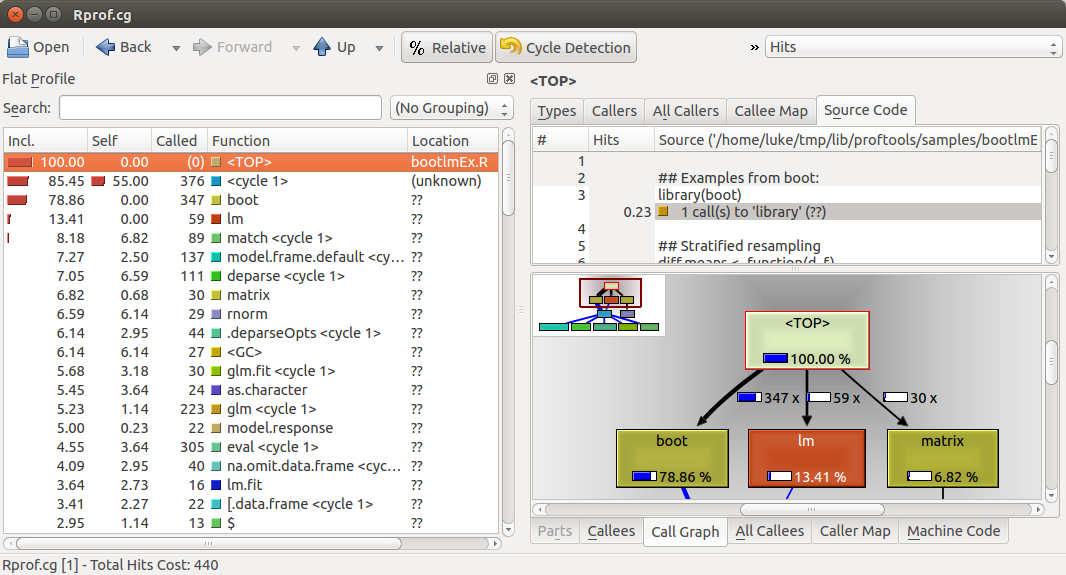
\includegraphics[width=\maxwidth]{kcachegrind}
  \caption{\code{kcachegrind} interface for examining profile data for
    the example.}
\label{kcachegrindFig}
\end{figure}
By default \code{writeCallgrindFile} for the common case where, as
here, the profiled code is in a file run using \code{source} and
source code information is retained. If this is the case,
\code{writeCallgrindFile} removes calls associated with the
\code{source} call and adds a \code{<TOP>} entry; this persuades
\code{kcachegrind} to show the top level line information.

Graphical user interfaces within R will be made available in the
\href{https://github.com/ltierney/Rpkg-proftools-GUI}{\pkg{proftoolsGUI}}
package. The current development version provides two interfaces, one
based on \pkg{gWidgets2} \citep{Verzani:gWidgets2} and one on
\pkg{shiny} \citep{Chang:shiny}.

\bibliography{proftools}
\end{document}
